% Wave Motions in the Ocean: Myrl's View
% Chapter 1; historical source: source/ChapmanRizzoli0_2.pdf.
% Source-page comments preserve printed/physical page correspondence.
% Substantive corrections are documented in ERRATA.md.

\setcounter{chapter}{0}
\setcounter{page}{1}

% -----------------------------------------------------------------------------
% Source printed page 1 / physical page 11
% -----------------------------------------------------------------------------
\chapter{Basic concepts}

Waves are not easy to define. Whitham (1974) defines a wave as ``a recognizable signal
that is transferred from one part of a medium to another with recognizable velocity of
propagation''. This is a very broad definition and encompasses an enormous range of
dynamical systems as well as physical processes. That is, waves can occur in many
different media and take on many different forms. We often think of waves as simple
sinusoidal undulations of some substance, but this view is too restricted and often not
very useful.

In this course, we will consider a number of different types of waves and wave motions
in the ocean and in the atmosphere. They will be found to occur at many different time
and space scales. In general, wave-like fluctuations of flow fields are not exact
solutions of the continuum formulation of momentum and mass conservation and the laws
of thermodynamics. However, they often represent good approximate solutions of those
equations.

\sourcepagebreak

% -----------------------------------------------------------------------------
% Source printed page 2 / physical page 12
% -----------------------------------------------------------------------------
Therefore, the first step in discussing wave motion is the appropriate simplification of
the field equations to obtain a set whose solutions are waves. In most of what we do,
this involves \emph{linearizing} the field equations about some basic state of rest or of
quasi-steady motion. That is, products of any dependent variables in the equations are
typically assumed to be small in relation to the other terms. It usually proves possible,
by this device, to obtain waves as solutions of the linearized equations.

Because the equations are linear, we are entitled to superpose solutions of the equations
in order to find solutions to more general initial and boundary value problems. This is
one of the real beauties of linear wave theory. We will spend most of our time studying
such linear waves and their properties before relaxing the linearization condition which
precludes nonlinear interactions.

As we will see, there are many different waves with quite different characteristics which
can exist within the framework of rotating fluid systems such as the ocean and the
atmosphere. In order to proceed, certain concepts and approaches which are common to
most studies of linear waves should be understood first. Some of these are presented
next.

\section{Plane waves}

The basic state of rest or quasi-steady flow about which the waves are linear
perturbations defines the medium through which the waves propagate. If we \emph{assume}
that the medium is homogeneous in space and time (even if it strictly is not), then
possible solutions often have the form of a \emph{plane wave}:
\[
 \phi(\vec{x},t)=\Re\,A e^{i(\vec{k}\cdot\vec{x}-\sigma t)}.
\]

\sourcepagebreak

% -----------------------------------------------------------------------------
% Source printed page 3 / physical page 13
% -----------------------------------------------------------------------------
where $\phi(\vec{x},t)$ are the dependent variables (i.e., velocity $\vec{u}$, pressure
$p$, density $\rho$, etc.), $A$ is the amplitude, $\vec{k}=(k,\ell,m)$ is the
wavenumber, $\sigma$ is the radian frequency, and $\Re$ means that we take the real
part of the expression. Customary auxiliary definitions are
\[
 \lambda=2\pi/|\vec{k}|=\text{wavelength},\qquad
 f=\sigma/2\pi=\text{frequency},\qquad
 T=2\pi/\sigma=1/f=\text{period}.
\]

Since $A$ is complex, it carries with it not only amplitude but also phase information.
We could, of course, write
\[
 \phi(\vec{x},t)=|A|\cos\left(\vec{k}\cdot\vec{x}-\sigma t
 +\arg A\right)
\]
where $\arg A$ denotes the complex argument of $A$. However, it is often much
more convenient to work with the complex form of all variables and to take the real
parts only at the very end. This is always possible because we have linearized the field
equations.

The convention $e^{i(\vec{k}\cdot\vec{x}-\sigma t)}$ is preferable to the convention
$e^{i(\vec{k}\cdot\vec{x}+\sigma t)}$ because, in the first case, wave `crests and
troughs' move in the direction of $\vec{k}$ when $\sigma>0$. This can be seen by
examining the \emph{phase} of the wave, namely $\vec{k}\cdot\vec{x}-\sigma t$.
Surfaces of constant phase, $\vec{k}\cdot\vec{x}-\sigma t=\Phi_0$, are planes normal
to $\vec{k}$ and moving outward along $\vec{k}$ as $t$ increases (for $\sigma>0$).
In two dimensions we have

\sourcepagebreak

% -----------------------------------------------------------------------------
% Source printed page 4 / physical page 14
% -----------------------------------------------------------------------------
\par\smallskip
\begin{center}
% wave-source: pdf=ChapmanRizzoli0_2.pdf; page=14; trim=60.24bp 443.04bp 78.72bp 36.00bp
% Source: Wave Motions in the Ocean, printed p.4 (physical p.14).
% Equation-constrained vector reconstruction of the original phase-plane sketch.
% The parallel phase planes are normal to the wavevector. Their separation along
% the wavevector is one wavelength, lambda = 2 pi / |kbar|. Geometry is schematic;
% the display angle theta=35 deg is chosen only to match the source drawing.
\begin{tikzpicture}[x=0.88cm,y=0.88cm,>=stealth,line cap=round,line join=round,font=\small]
  \def\ang{35}
  \def\sone{1.90}
  \def\stwo{3.80}
  \def\kend{6.20}
  \coordinate (O) at (0,0);
  \coordinate (K) at ({\kend*cos(\ang)},{\kend*sin(\ang)});
  \coordinate (Kx) at ({\kend*cos(\ang)},0);

  % Cartesian axes and wavevector components.
  \draw[->,line width=0.78pt] (O) -- (8.25,0) node[right] {$x$};
  \draw[->,line width=0.78pt] (O) -- (0,5.55) node[above] {$y$};
  \draw[->,line width=1.02pt] (O) -- (K);
  \draw[dashed,line width=0.58pt] (K) -- (Kx);
  \node[above=2pt] at (K) {$\bar{k}$};
  \node[below=2pt] at (Kx) {$k$};
  \node[right=4pt] at ($(K)!0.50!(Kx)$) {$\ell$};

  % theta is the angle from the x axis to the wavevector.
  \draw[line width=0.52pt] (0.92,0) arc[start angle=0,end angle=\ang,radius=0.92];
  \node at (1.12,0.36) {$\theta$};

  % Work in the orthogonal (along-k, phase-plane) frame. Local x is parallel
  % to the wavevector; local y is tangent to the constant-phase planes.
  \begin{scope}[rotate=\ang]
    % kx + ell y - sigma t = constant: three parallel constant-phase planes.
    \draw[line width=0.76pt] (0,-1.55) -- (0,4.05);
    \draw[line width=0.76pt] (\sone,-1.55) -- (\sone,3.45);
    \draw[line width=0.76pt] (\stwo,-1.70) -- (\stwo,3.00);

    % Right-angle marks emphasize that phase planes are normal to the wavevector.
    \foreach \s in {0,\sone,\stwo} {
      \draw[line width=0.50pt]
        (\s+0.20,0) -- (\s+0.20,0.20) -- (\s,0.20);
    }

    % The source uses small wavy propagation arrows normal to two phase planes.
    \foreach \s in {\sone,\stwo} {
      \draw[->,line width=0.58pt,samples=55,domain=-0.68:0.55,variable=\q]
        plot ({\s+\q},{0.38+0.075*sin(900*\q)});
    }

    % One wavelength is the normal distance between adjacent phase planes.
    \draw[decorate,decoration={brace,amplitude=4.2pt,mirror},line width=0.52pt]
      (0.18,-1.27) -- (\sone-0.18,-1.27);
    \node[anchor=north west] at (1.15,-1.63)
      {$\lambda=\dfrac{2\pi}{|\bar{k}|}$};
  \end{scope}

  % Source labels lie along the upper-left portions of the first two planes.
  \node[rotate={\ang-90},anchor=south,inner sep=1.5pt] at
    ({-1.95*sin(\ang)},{1.95*cos(\ang)})
    {$kx+\ell y-\sigma t=0$};
  \node[rotate={\ang-90},anchor=east,inner sep=1.5pt] at (-0.62,3.72)
    {$kx+\ell y-\sigma t=2\pi$};
\end{tikzpicture}

\wavefiguremark
\end{center}
\smallskip

The speed at which phase planes move normal to themselves is the \emph{phase speed}
\[
 c=\sigma/|\vec{k}|=\lambda/T.
\]
For the stated $\sigma>0$ convention the associated normal phase-velocity vector is
$\vec c_p=c\,\hat{\vec k}=\sigma\vec k/|\vec k|^2$. Note that the speed of phase plane intersection with the
$x$-axis is not $c\cos\theta$ but rather is
\[
 \frac{c}{\cos\theta}
 =\left(\frac{\sigma}{|\vec{k}|}\right)
  \left(\frac{|\vec{k}|}{k}\right)
 =\sigma/k
\]
which can be considerably faster than $c$. In fact, as $\theta\to\pi/2$, the phase
speed in the $x$-direction approaches infinity!

The form $Ae^{i(\vec{k}\cdot\vec{x}-\sigma t)}$ is called a `travelling plane wave'.
The superposition of oppositely travelling plane waves
\[
 Ae^{i(\vec{k}\cdot\vec{x}-\sigma t)}
 +Ae^{i(-\vec{k}\cdot\vec{x}-\sigma t)}
 =2Ae^{-i\sigma t}\cos(\vec{k}\cdot\vec{x})
\]
is called a \emph{standing wave} because the crests and troughs do not propagate with
time. It is not always possible to construct such a superposition because oppositely
travelling plane waves are not always possible and, even when possible, may have
different wavenumbers.

\sourcepagebreak

% -----------------------------------------------------------------------------
% Source printed page 5 / physical page 15
% -----------------------------------------------------------------------------
\section{The dispersion relation}

All of the foregoing is kinematics, true for any given $\sigma,\vec{k}$ with no physics.
The physics are contained in the \emph{dispersion relation}
\[
 \sigma=\Omega(\vec{k})
\]
which is obtained by requiring the plane waves to be solutions of the linearized,
dissipationless equations of motion. The following table contains some examples of wave
equations (all of which we will encounter later) with their respective dispersion
relations.

\begin{center}
\begin{tabular}{c@{\quad}l@{\quad}l@{\quad}l}
 & Linearized Equation & Plane wave & Dispersion Relation\\[3pt]
 a) & $\phi_t+c_0\phi_x=0$
    & $e^{ikx-i\sigma t}$ & $\sigma=c_0k$\\
 b) & $\phi_{tt}-c_0^2\phi_{xx}=0$
    & $e^{ikx-i\sigma t}$ & $\sigma^2=c_0^2k^2$\\
 c) & $\phi_t+\vec c_0\cdot\nabla\phi=0$
    & $e^{i\vec{k}\cdot\vec{x}-i\sigma t}$
    & $\sigma=\vec c_0\cdot\vec{k}$\\
 d) & $\phi_{tt}-c_0^2\nabla^2\phi=0$
    & $e^{i\vec{k}\cdot\vec{x}-i\sigma t}$
    & $\sigma^2=c_0^2|\vec{k}|^2$\\
 e) & $\nabla^2\phi_t+\beta\phi_x=0$
    & $e^{i\vec{k}\cdot\vec{x}-i\sigma t}$
    & $\sigma=-\beta k/|\vec{k}|^2$
\end{tabular}
\end{center}

Each linearized equation is a statement of approximate dynamical and thermodynamical
conservation laws. All are solved using plane waves of the type discussed above. All
require different dispersion relations, and the solutions have different properties. For
cases (a), (b), and (d), the phase speed $c=\sigma/|\vec{k}|$ is independent
of wavelength, frequency or direction. In case (c),
$c=\vec c_0\cdot\hat{\vec k}$, so the phase speed is independent of wavelength and
frequency but depends on propagation direction relative to $\vec c_0$. For any fixed
propagation direction, cases (a)--(d) are nondispersive with respect to wavenumber
magnitude. In case (e), the phase speed $c$ is dependent upon the wavelength and the
direction, so these waves are dispersive. As we will see, this basically means that a group of such

\sourcepagebreak

% -----------------------------------------------------------------------------
% Source printed page 6 / physical page 16
% -----------------------------------------------------------------------------
waves will not remain together while propagating through the medium, but instead will
break up or disperse. Standing waves, as defined above, are possible in cases (b) and
(d) because oppositely travelling waves can occur with the same wavenumber but with
frequencies of opposite sign. That is, the dispersion relation has more than one branch,
$\sigma=\Omega_j(\vec{k})$ for $j=1,\ldots,n$. However, in cases (a), (c) and (e), a
given wavenumber corresponds to only a single frequency (only one branch), i.e. waves
can travel only in one direction, so standing waves are not possible.

Several cautionary notes are in order here. Plane waves are rarely the complete solution
to any boundary or initial value problem. If the medium is actually homogeneous and
steady, then plane waves may often be superposed to solve such problems. However,
often the medium is not homogeneous or steady, so plane wave solutions then require
modifications before they can be used. We shall spend a good part of this course
deriving linearized equations which isolate particular physics and we shall discuss the
appropriate plane wave solutions in detail. But it must be kept in mind that, in order
to establish a basis for comparison with observations of real systems, a boundary or
initial value problem must be solved, most probably including medium inhomogeneities.
We shall, in some instances, show examples of such problems for some sets of linearized
equations.

\section{Linear superposition of plane waves}

In a homogeneous medium, initial value problems are solvable as Fourier integrals which
amounts to summing an infinite number of plane wave solutions. If the dispersion
relation has $n$ branches
\[
 \sigma=\Omega_j(\vec{k}),\qquad j=1,\ldots,n
\]

\sourcepagebreak

% -----------------------------------------------------------------------------
% Source printed page 7 / physical page 17
% -----------------------------------------------------------------------------
then $n$ initial conditions are normally required. The solution takes the form
\[
 \phi(\vec{x},t)=\sum_{j=1}^n
 \iiint_{-\infty}^{\infty}
 A_j(\vec{k})e^{i[\vec{k}\cdot\vec{x}-\Omega_j(\vec{k})t]}
 \,d\vec{k}
\]
where the $A_j(\vec{k})$ are fixed by the initial conditions. For example, if $n=1$,
and we are in one dimension
\[
 \sigma=\Omega(k)
\]
\[
 \phi(x,t)=\int_{-\infty}^{\infty}
 A(k)e^{i[kx-\Omega(k)t]}
 \,dk.
\]
$A(k)$ is fixed by specifying $\phi(x,0)$, that is
\[
 \phi(x,0)=\int_{-\infty}^{\infty}A(k)e^{ikx}\,dk;
 \qquad
 A(k)=\frac{1}{2\pi}\int_{-\infty}^{\infty}\phi(x,0)e^{-ikx}\,dx.
\]
Notice that if $\Omega=ck$, then
\[
 \phi(x,t)=\int_{-\infty}^{\infty}A(k)e^{ik(x-ct)}\,dk
 =\int_{-\infty}^{\infty}A(k)e^{ikx'}\,dk
 =\phi(x-ct,0).
\]
This means that, in this special case, the initial condition $\phi(x,0)$ translates
towards $x>0$ at speed $c$ without changing shape.

For homogeneous media, therefore, the problem is generally solved by (i) finding the
dispersion relation, (ii) deducing the $A_j(\vec{k})$ from initial conditions, and (iii)
evaluating a set of Fourier integrals.

\section{The method of stationary phase: Group velocity}

The greatest difficulty with the above procedure is most often that the integrals are
hard to do. A very useful approximate technique with physical content is the method

\sourcepagebreak

% -----------------------------------------------------------------------------
% Source printed page 8 / physical page 18
% -----------------------------------------------------------------------------
of stationary phase. As a preview, let us consider a one-dimensional example with the
special initial condition $\phi(x,0)=a(x)e^{ik_0x}$.

\par\smallskip
\begin{center}
% wave-source: pdf=ChapmanRizzoli0_2.pdf; page=18; trim=113.04bp 486.00bp 72.00bp 132.00bp
% Vector redraw of the modulated plane-wave packet on printed page 8.
% Source: ChapmanRizzoli0_2.pdf, physical page 18.
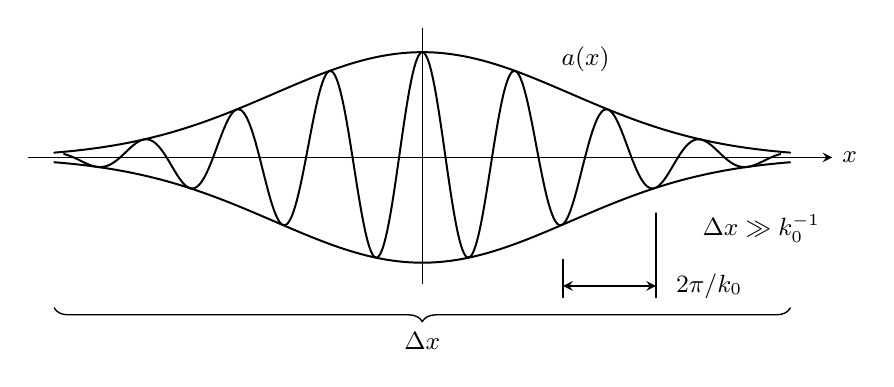
\begin{tikzpicture}[x=0.82cm,y=0.82cm,>=stealth,line cap=round,line join=round,font=\small]
  % Horizontal coordinate axis.
  \draw[->,line width=0.55pt] (-6.1,0) -- (6.35,0) node[right] {$x$};

  % Slowly varying envelope a(x), drawn symmetrically about the axis.
  \draw[line width=0.72pt,samples=121,smooth,domain=-5.7:5.7]
    plot (\x,{1.63*exp(-0.095*\x*\x)});
  \draw[line width=0.72pt,samples=121,smooth,domain=-5.7:5.7]
    plot (\x,{-1.63*exp(-0.095*\x*\x)});
  \node[above right=-1pt] at (2.05,1.22) {$a(x)$};

  % Carrier oscillation, with the same Gaussian envelope.
  \draw[line width=0.72pt,samples=260,smooth,domain=-5.55:5.55]
    plot (\x,{1.63*exp(-0.095*\x*\x)*cos(250*\x)});

  % Central reference line as in the source sketch.
  \draw[line width=0.45pt] (0,-1.95) -- (0,2.00);

  % One wavelength indicator under the positive-x carrier.
  \draw[line width=0.45pt] (2.18,-1.58) -- (2.18,-2.17);
  \draw[line width=0.45pt] (3.62,-0.86) -- (3.62,-2.17);
  \draw[<->,line width=0.55pt] (2.18,-1.99) -- (3.62,-1.99);
  \node[anchor=west] at (3.78,-1.99) {$2\pi/k_0$};

  % Packet-width brace and labels.
  \draw[decorate,decoration={brace,amplitude=5pt,mirror},line width=0.50pt]
    (-5.70,-2.33) -- (5.70,-2.33);
  \node at (0,-2.84) {$\Delta x$};
  \node at (5.25,-1.10) {$\Delta x\gg k_0^{-1}$};
\end{tikzpicture}

\wavefiguremark
\end{center}
\smallskip

This represents a slowly modulated plane wave with envelope $a(x)$. We can always
write
\[
 \phi(x,0)=\int_{-\infty}^{\infty}A(k)e^{ikx}\,dk;
 \qquad
 A(k)=\frac{1}{2\pi}\int_{-\infty}^{\infty}\phi(x,0)e^{-ikx}\,dx
\]
and so
\[
 A(k)=\frac{1}{2\pi}\int_{-\infty}^{\infty}
 a(x)e^{i(k_0-k)x}\,dx;
 \qquad
 a(x)=\int_{-\infty}^{\infty}A(k)e^{i(k-k_0)x}\,dk.
\]
In the integral for $A(k)$, the contribution to the integral itself is mostly from the
regions where the quantity $(k_0-k)x$ is small. In fact, where this quantity is large,
$e^{i(k_0-k)x}$ oscillates rapidly and the integrated parts cancel each other. Moreover,
$a(x)=0$ for $x\gg\Delta x$. So, $A(k)$ is centered around $k_0$ and peaked there for
this special choice of $\phi(x,0)$.

\par\smallskip
\begin{center}
% wave-source: pdf=ChapmanRizzoli0_2.pdf; page=18; trim=178.08bp 100.08bp 207.84bp 517.92bp
% Vector redraw of the narrow-band spectrum on printed page 8.
% Source: ChapmanRizzoli0_2.pdf, physical page 18.
\begin{tikzpicture}[x=0.82cm,y=0.82cm,>=stealth,line cap=round,line join=round]
  % Axes as in the original sketch; the vertical axis extends slightly below k=0.
  \draw[line width=0.58pt] (-0.18,0) -- (6.10,0);
  \draw[line width=0.58pt] (0,-0.62) -- (0,4.65);
  \node[anchor=east] at (-0.28,2.05) {$A(k)$};

  % Narrow-band spectral amplitude centered on k_0.
  \draw[line width=0.78pt,samples=140,smooth,domain=0:5.65]
    plot (\x,{0.10 + 3.52*exp(-0.72*(\x-2.95)*(\x-2.95))});

  % k_0 marker.
  \draw[line width=0.48pt] (2.95,0) -- (2.95,-0.55);
  \node[below] at (2.95,-0.50) {$k_0$};
\end{tikzpicture}

\wavefiguremark
\end{center}
\smallskip

The modulated plane wave is said to be a `narrow band signal'.

\setcounter{page}{9}

% -----------------------------------------------------------------------------
% Source printed page 9 / physical page 19
% -----------------------------------------------------------------------------
We can evaluate $\phi(x,t)$ by expanding $\Omega(k)$ in a Taylor series about $k_0$:
\begin{align*}
 \phi(x,t)
 &=\int_{-\infty}^{\infty}A(k)e^{i[kx-\Omega(k)t]}\,dk\\
 &\simeq\int_{-\infty}^{\infty}A(k)
 e^{i[kx-\Omega(k_0)t-(k-k_0)(\partial\Omega/\partial k)|_{k=k_0}t]}\,dk\\
 &=\int_{-\infty}^{\infty}A(k)
 e^{i[kx-\Omega(k_0)t-(k-k_0)(\partial\Omega/\partial k)|_{k=k_0}t]}
 e^{ik_0x-ik_0x}\,dk\\
 &=e^{i[k_0x-\Omega(k_0)t]}
 \int_{-\infty}^{\infty}A(k)
 e^{i(k-k_0)[x-(\partial\Omega/\partial k)|_{k=k_0}t]}\,dk.
\end{align*}
That is
\[
 \phi(x,t)=e^{i[k_0x-\Omega(k_0)t]}
 a\left(x-\left.\frac{\partial\Omega}{\partial k}\right|_{k=k_0}t\right).
\]
The modulating envelope moves at a velocity
$\left.\partial\Omega/\partial k\right|_{k=k_0}$, defined by the dispersion relation
$\sigma=\Omega(k)$. This velocity is called the \emph{group velocity}
\[
 c_g=\left.\frac{\partial\Omega}{\partial k}\right|_{k=k_0}
\]
and is not, in general, equal to the phase speed $c=\sigma/k$ of the modulated plane
wave. Therefore, the dominant wavelength $\lambda=2\pi/k_0$ has two speeds associated
with it. They are the phase speed $c=\sigma/k_0=\Omega(k_0)/k_0$ and the group
velocity $c_g=\partial\sigma/\partial k|_{k=k_0}=\partial\Omega/\partial k|_{k=k_0}$.
The modulated envelope thus moves \emph{through} the phases of the underlying plane
wave rather than with them.

The restriction to narrow band processes is illustrative but not necessary. Consider
\[
 \phi(x,t)=\int_{-\infty}^{\infty}A(k)e^{i[kx-\Omega(k)t]}\,dk.
\]
Define
\[
 \Theta(k;x,t)=kx/t-\Omega(k).
\]
Then
\[
 \phi(x,t)=\int_{-\infty}^{\infty}A(k)e^{it\Theta(k;x,t)}\,dk.
\]

\sourcepagebreak

% -----------------------------------------------------------------------------
% Source printed page 10 / physical page 20
% -----------------------------------------------------------------------------
The Riemann--Lebesgue theorem (e.g. Bender and Orszag, 1978, pp. 277--278) says that
if $\int_{-\infty}^{\infty}A(k)\,dk$ exists, then
$\lim_{t\to\infty}\int_{-\infty}^{\infty}A(k)e^{itk}\,dk=0$. Hence, we get little
contribution to $\phi(x,t)$ unless $\Theta(k;x,t)$ has no variation with $k$, i.e.,
unless there exist $k_0$ such that
$\left.(\partial\Theta/\partial k)\right|_{k_0}=0$. Perhaps a more intuitive statement
is that the integrand looks like

% Vector reconstruction; source PDF ChapmanRizzoli0_2.pdf, physical page 20, trim=84bp 481bp 117bp 202bp.
\wavevectorart[0.76]{ch01-p010-stationary-phase}

in which the rapid oscillations of $e^{it\Theta}$, as $t\to\infty$, cancel unless
$\partial\Theta/\partial k=0$ somewhere.

Stationary phase now asserts
\[
 \phi(x,t)\simeq\int_{-\infty}^{\infty}A(k)
 e^{it[\Theta(k_0)+(k-k_0)\Theta'(k_0)
 +(k-k_0)^2\Theta''(k_0)/2]}\,dk.
\]
In other words, at a given $x$ and $t$, the greatest contribution to $\phi(x,t)$ is from
that wavenumber $k_0$ at which $\Theta'(k_0;x,t)=0$. Since
$\Theta(k;x,t)=kx/t-\Omega(k)$ we have
\[
 x/t-\left.\frac{\partial\Omega}{\partial k}\right|_{k_0}=0
\]
which means that the wavenumber $k_0$ that makes the biggest contribution to
$\phi(x,t)$ is the one for which
\[
 \left.\frac{\partial\Omega}{\partial k}\right|_{k_0}=x/t;
\]
i.e., the one whose group velocity is $x/t$.

To estimate that contribution, realise that $\Theta'(k_0)=0$, so that
\[
 \phi(x,t)\simeq A(k_0)e^{it\Theta(k_0)}
 \int_{-\infty}^{\infty}
 e^{i(k-k_0)^2\Theta''(k_0)t/2}\,dk.
\]

\sourcepagebreak

% -----------------------------------------------------------------------------
% Source printed page 11 / physical page 21
% -----------------------------------------------------------------------------
or, since $\int_{-\infty}^{\infty}e^{-\alpha x^2}\,dx=(\pi/\alpha)^{1/2}$, then
\[
 \phi(x,t)\simeq A(k_0)e^{it\Theta(k_0)}
 [2\pi/-it\Theta''(k_0;x,t)]^{1/2}
\]
\[
 \phi(x,t)\simeq A(k_0)e^{i[k_0x-\Omega(k_0)t]}
 [2\pi/-it\Theta''(k_0;x,t)]^{1/2}.
\]
The solution is thus a slowly modulated plane wave whose wavenumber $k_0$ is
characterized by
\[
 \left.\frac{\partial\Omega}{\partial k}\right|_{k_0}=x/t.
\]

The solution is only valid for very large $t$ and $x$ because it requires the rapid
oscillation of $e^{i[kx-\Omega(k)t]}$ at all $k$ except those where
$x-\Omega_k t=0$. It thus describes the waves far from and long after their initial
generation.

\section{Waves in slowly varying media: Ray theory}

The procedure of Fourier synthesis followed by stationary phase interpretation is
natural in homogeneous media. It introduces the concept of group velocity, but the idea
and significance of group velocity extend into problems for which Fourier synthesis is
clumsy at best. An important set of such problems includes those for which the medium
varies over a scale $L_m$ which is much greater than the length scale of the waves,
$L_w$. In these cases, an approximate technique called the WKB method can exploit the
smallness of $L_w/L_m$. The WKB method, however, is often tedious and difficult to
interpret. Instead, a general `recipe' called \emph{ray theory}, which corresponds to the
first and second orders of approximation of the WKB method, can be used.

Let us consider a locally periodic solution of the form
\[
 \phi=a(\vec{x},t)e^{i\Theta(\vec{x},t)}
\]
in which the amplitude $a$ and the local wave parameters vary slowly, while the phase
$\Theta$ itself varies on the wave scale. More precisely, $a$ and the derivatives of
$\Theta$ change with the large space and time scales of the medium or of the wave groups

\sourcepagebreak

% -----------------------------------------------------------------------------
% Source printed page 12 / physical page 22
% -----------------------------------------------------------------------------
and not the small scale of the sinusoidal plane wave. We can define the local
wavenumber $\vec{k}$ and the local frequency $N$ by
\[
 \vec{k}=\left.\nabla\Theta\right|_t;
 \qquad
 N=-\left.\Theta_t\right|_{\vec{x}}
\]
where $\nabla$ is the gradient operator and $|_t$, $|_{\vec{x}}$ indicate that the
partial derivatives are carried out keeping the other coordinate constant. The WKB
assumption is that $a$, $\vec{k}$, and $N$ change only by small fractions over local
distances and times of order $|\vec{k}|^{-1}$ and $|N|^{-1}$; $\Theta$ itself need not
vary slowly.

For these definitions, we see first that
\[
 \nabla\times\vec{k}=0
\]
which states that the local wavenumber is irrotational. Now suppose we go from place
$A$ to place $B$ over the path $\Gamma$.

% Vector reconstruction; source PDF ChapmanRizzoli0_2.pdf, physical page 22, trim=175bp 328bp 235bp 324bp.
\wavevectorart[0.43]{ch01-p012-wave-crest-path}

The number of wave crests we pass through is
\[
 n=\frac{1}{2\pi}\int_A^B\vec{k}\cdot d\vec{s}.
\]
But since
$\oint\vec{k}\cdot d\vec{s}=\int\hat{k}\cdot\nabla\times\vec{k}\,dr=0$
(by Stokes' theorem where $\hat{k}$ is the unit vector normal to the surface and $dr$
is an element of the area inside the path), then the number of wave crests inside the
region is conserved. That is, the crests have no ends, so the number of crests within a
wave group will be the same for all time. This need not be true for all waves, but it is
true for slowly varying plane waves as defined above.

\sourcepagebreak

% -----------------------------------------------------------------------------
% Source printed page 13 / physical page 23
% -----------------------------------------------------------------------------
From the definition of $\vec{k}$ and $N$, it follows that
\begin{equation}
 \left.\frac{\partial\vec{k}}{\partial t}\right|_{\vec{x}}
 +\left.\nabla N\right|_t=0.
 \tag{1.1}
\end{equation}
Now with the above definition of $n$, we have
\[
 \frac{\partial n}{\partial t}
 =\frac{1}{2\pi}\int_A^B\frac{\partial\vec{k}}{\partial t}\cdot d\vec{s}
 =-\frac{1}{2\pi}\int_A^B\nabla N\cdot d\vec{s}
 =\frac{1}{2\pi}(N_A-N_B).
\]
This says that the rate of change of the number of wave crests between $A$ and $B$ is
equal to the rate of crest inflow at $A$ minus the rate of crest outflow at $B$. Thus
(1.1) expresses the conservation of wave crests between $A$ and $B$, i.e., crests are
neither created nor destroyed.

So far, we have defined the local wavenumber and frequency only as derivatives of
$\Theta$. There has been no direct statement of dynamics. We introduce dynamics by
asserting that the wavenumber and frequency must be related in just the same way that
they are for a plane wave!
\[
 N=\Omega(\vec{k};\vec{x},t)
\]
where, if we solved for plane waves $e^{i(\vec{k}\cdot\vec{x}-\sigma t)}$ while keeping
all variable medium parameters momentarily constant, we would obtain
$\sigma=\Omega(\vec{k};\vec{x},t)$ as our dispersion relation. This turns out to be
equivalent to the lowest order of a WKB calculation, despite being stated here as an
arbitrary recipe.

Now this assertion and the definitions of $\vec{k}$ and $N$ allow us to introduce the
group velocity in another way.
\[
 \left.\frac{\partial N}{\partial t}\right|_{\vec{x}}
 =\left.\frac{\partial\Omega}{\partial t}\right|_{\vec{k},\vec{x}}
 +\left.\frac{\partial\Omega}{\partial k_i}\right|_{\vec{x},t}
  \left.\frac{\partial k_i}{\partial t}\right|_{\vec{x}}
 =\left.\frac{\partial\Omega}{\partial t}\right|_{\vec{k},\vec{x}}
 -c_{g_i}\left.\frac{\partial N}{\partial x_i}\right|_t
\]
in which the group velocity has been defined as
\[
 c_{g_i}=\frac{\partial N}{\partial k_i}=\frac{\partial\Omega}{\partial k_i}.
\]

\sourcepagebreak

% -----------------------------------------------------------------------------
% Source printed page 14 / physical page 24
% -----------------------------------------------------------------------------
and the repeated index implies summation. In vector form, we have
\begin{equation}
 \frac{\partial N}{\partial t}+\vec{c}_g\cdot\nabla N
 =\left.\frac{\partial\Omega}{\partial t}\right|_{\vec{k},\vec{x}}.
 \tag{1.2}
\end{equation}
In a similar manner starting with (1.1)
\[
 \frac{\partial k_i}{\partial t}
 +\frac{\partial\Omega}{\partial x_i}
 +\frac{\partial\Omega}{\partial k_j}
  \frac{\partial k_j}{\partial x_i}=0.
\]
Since $\nabla\times\vec{k}=0$, then
$\partial k_j/\partial x_i=\partial k_i/\partial x_j$, so we have
\begin{equation}
 \frac{\partial k_i}{\partial t}+\vec{c}_g\cdot\nabla k_i
 =-\left.\frac{\partial\Omega}{\partial x_i}\right|_{\vec{k},t}.
 \tag{1.3}
\end{equation}
We thus have very simple expressions, (1.2) and (1.3), for the evolution of local
wavenumber $\vec{k}$ and local frequency $N$ as we move along a ray (i.e., we move at
the local group velocity $\vec{c}_g$) in terms of the plane wave dispersion relation.
Such variations occur when $\Omega(\vec{k};\vec{x},t)$ has parametric $\vec{x},t$
dependence such as if waves move in water of variable depth.

The implications of these equations deserve some discussion. Suppose first that the
medium is homogeneous, i.e. $N=\Omega(\vec{k})\ne\Omega(\vec{k};\vec{x},t)$. One
possible solution is the plane wave
$\phi=ae^{i(\vec{k}\cdot\vec{x}-Nt)}$ when $\vec{k}$ and $N$ are constants. The
initial condition is $\phi(\vec{x},0)=ae^{i\vec{k}\cdot\vec{x}}$. Since
$\partial k_i/\partial x_j=0$ and $\partial\Omega/\partial x_i=0$, then from (1.3),
$\partial k_i/\partial t=0$ everywhere, that is $\vec{k}$ never changes at future times.
Similarly, $N=\Omega(\vec{k})$ gives $N$ at $t=0$. Since
$\partial N/\partial x_i=0$, $\partial\Omega/\partial t=0$, then by (1.2)
$\partial N/\partial t=0$ everywhere, that is $N$ never changes at future times. The
plane wave in a homogeneous medium is thus entirely consistent with the ray theory
formulation.

Suppose now that the medium remains homogeneous, but the initial conditions are more
complicated. Both $a$ and $\vec{k}$ have slow $\vec{x}$ dependence at $t=0$ as
illustrated below:

\sourcepagebreak

% -----------------------------------------------------------------------------
% Source printed page 15 / physical page 25
% -----------------------------------------------------------------------------
% Vector reconstruction; source PDF ChapmanRizzoli0_2.pdf, physical page 25, trim=62bp 445bp 69bp 46bp.
\wavevectorart[0.88]{ch01-p015-initial-wave-groups}

Notice that $a$ and $\vec{k}$ should vary slowly over $\lambda$, even though the sketch
is not very slowly varying.

The initial frequency is obtained from
$N(\vec{x},0)=\Omega[\vec{k}(\vec{x},0)]$. To find
$N(\vec{x},t)$, $\vec{k}(\vec{x},t)$ we solve the initial value problem
\[
 \frac{\partial k_i}{\partial t}
 +c_{g_j}\frac{\partial k_i}{\partial x_j}=0
\]
\[
 \frac{\partial N}{\partial t}
 +c_{g_j}\frac{\partial N}{\partial x_j}=0
\]
because the assumed homogeneity of the medium implies
$\partial\Omega/\partial t=0$ and $\partial\Omega/\partial x_i=0$. This initial value
problem may have to be solved numerically, but the equations have a simple physical
interpretation. They say that, if we move at the group velocity
$\vec{c}_g=\nabla_{\vec{k}}\Omega$ appropriate to the wavenumber $\vec{k}$ and the
frequency $N=\Omega(\vec{k})$, then we shall see no change in $N$ and $\vec{k}$ at
future times. In other words, $N$ and $\vec{k}$ are constant following a group in a
homogeneous medium. The situation can be sketched as follows

\sourcepagebreak

% -----------------------------------------------------------------------------
% Source printed page 16 / physical page 26
% -----------------------------------------------------------------------------
% Vector reconstruction; source PDF ChapmanRizzoli0_2.pdf, physical page 26, trim=62bp 450bp 69bp 46bp.
\wavevectorart[0.88]{ch01-p016-ray-crossing}

Clearly, if we sit at a fixed $\vec{x}$, different groups pass at different times. So at
fixed $\vec{x}$, $\partial N/\partial t\ne0$, $\partial\vec{k}/\partial t\ne0$, in
general, even though the medium is homogeneous. The whole idea fails if the rays,
given by
\[
 \vec{x}=\vec{x}_0+
 \int_0^t\vec{c}_g[\vec{k}(\vec{x},t)]\,dt
\]
cross each other. In that case, the solution is no longer of slowly varying form.

From this point of view, the medium inhomogeneities are only technical complications.
In the general inhomogeneous case, we must solve (1.2) and (1.3), so $\vec{k}$ and $N$
vary even though we move with a group. If we define a `total' derivative as
\[
 \frac{d}{dt}=\frac{\partial}{\partial t}+\vec{c}_g\cdot\nabla
\]
which is the derivative following the wave group (or wave packet), then (1.2) and (1.3)
can be rewritten as
\[
 \frac{dk_i}{dt}=-\frac{\partial\Omega}{\partial x_i}
\]
and
\[
 \frac{dN}{dt}=\frac{\partial\Omega}{\partial t}.
\]

\sourcepagebreak

% -----------------------------------------------------------------------------
% Source printed page 17 / physical page 27
% -----------------------------------------------------------------------------
while the position of the wave group is given by
\[
 \frac{d\vec{x}}{dt}=\vec{c}_g[\vec{k}(\vec{x},t)].
\]
Then we have a set of three ordinary differential equations for $\vec{x}$ (position of
the wave packet), $\vec{k}$ and $N$. These may be integrated in time from a number of
different starting positions $\vec{x}_0$ in order to get $\vec{k}$, $N$ at future times,
a procedure which is computationally efficient and effective. The path
$d\vec{x}/dt=\vec{c}_g$ defines the ray.

The lowest order of the corresponding WKB calculation justifies the foregoing
assertions. The next order of the WKB calculation fixes the amplitude. In many cases,
the more complex WKB calculation amounts to solving
\[
 \frac{\partial\mathcal{A}}{\partial t}
 +\nabla\cdot(\vec{c}_g\mathcal{A})=0
\]
where $\mathcal{A}=\mathcal{E}/N$ and $\mathcal{E}$ is the wave energy. $\mathcal{A}$
is called the \emph{action} of the wave. Usually $\mathcal{E}\propto a^2$ so this
equation really describes $a$, but a great deal of further discussion is necessary to
establish its validity. Here we have simply set forward `recipes' which give $a$, $N$,
$\vec{k}$.
